\documentclass[11pt,a4paper]{article}

% Packages
\usepackage[utf8]{inputenc}
\usepackage[T1]{fontenc}
\usepackage{graphicx}
\usepackage{booktabs}
\usepackage{amsmath}
\usepackage{amssymb}
\usepackage{hyperref}
\usepackage{geometry}
\usepackage{float}
\usepackage{caption}
\usepackage{subcaption}
\usepackage{tikz}
\usetikzlibrary{shapes,arrows,positioning}

\geometry{margin=1in}

% Title
\title{\textbf{Emergent Symbol Systems and Cultural Memory\\in a Self-Organizing Artificial Civilization}}
\author{
    \textbf{Sanchay Kumar}\\
    \texttt{ysanchay@gmail.com}\\
    \url{https://github.com/ysanchay/civilization-simulator}
}
\date{February 2026}

\begin{document}

\maketitle

\begin{abstract}
We present an experimental framework for studying the emergence of symbolic systems, cultural memory, and civilizational dynamics in decentralized multi-agent systems. Our simulator implements tribes of agents that inhabit a dynamic grid world, form symbols from perceived patterns, and develop predictive, causal, and goal-oriented representations. We demonstrate that language composition emerges spontaneously when symbol vocabularies exceed a transition threshold, and meta-symbol abstraction forms through co-occurrence tracking across tribes. The system implements cultural forgetting and compression mechanisms that drive abstraction under memory pressure. Critically, we measure knowledge independently of behavior through artifact structures—knowledge-only objects that agents can observe but that provide no direct survival reward. Our experiments reveal four key empirical findings: (1) war frequency follows a heavy-tailed distribution with kurtosis 11.59, indicating clustered conflict dynamics; (2) collapse events cluster into four distinct archetypes with different causal signatures; (3) symbolic complexity exhibits open-ended growth with a 4.62x increase over 1500 simulation steps; and (4) knowledge retention across simulation runs averages 41\%, improving with repeated exposure. We introduce three theoretical contributions: the Cultural Compression Hypothesis (memory pressure drives abstraction), the Predictive Survival Hypothesis (temporal prediction correlates with survival), and the Symbol Competition Hypothesis (meta-symbols replace base representations). These findings contribute to our understanding of emergent complexity in multi-agent systems and provide a controlled testbed for AI safety research on value emergence and civilizational stability.

\textbf{Keywords:} multi-agent systems, emergent behavior, symbolic grounding, cultural evolution, civilizational collapse, AI safety, language emergence, abstraction
\end{abstract}

\section{Introduction}

\subsection{Motivation}

How do civilizations emerge? This question has fascinated philosophers, historians, and scientists for centuries. Recent advances in multi-agent systems and artificial intelligence provide new tools for empirical investigation. By constructing artificial societies with minimal assumptions, we can observe emergent phenomena and test hypotheses about civilizational dynamics.

This work presents a civilization simulator designed to study:

\begin{enumerate}
    \item \textbf{Symbol Grounding}: How do abstract symbols emerge from grounded perception?
    \item \textbf{Cultural Memory}: How is knowledge preserved and transmitted across generations?
    \item \textbf{Civilizational Collapse}: What causes societies to fail, and can we predict it?
    \item \textbf{Open-Ended Evolution}: Does complexity grow indefinitely or saturate?
\end{enumerate}

\subsection{Why Current RL Systems Lack Cultural Continuity}

Standard reinforcement learning systems suffer from fundamental limitations when it comes to cultural evolution:

\begin{itemize}
    \item \textbf{Fixed Reward Functions}: RL agents optimize predetermined objectives, precluding the emergence of novel goals or values
    \item \textbf{No Memory Persistence}: Each episode typically resets state, eliminating the possibility of cumulative cultural knowledge
    \item \textbf{Isolation}: Agents learn independently without mechanisms for knowledge transfer
    \item \textbf{No Abstraction}: Representations remain at the level of sensory input, without symbol formation or composition
\end{itemize}

These limitations make standard RL unsuitable for studying how cultures form, evolve, and transmit knowledge across generations.

\subsection{Why Symbol Emergence Matters}

Symbol systems are the foundation of intelligent behavior:

\begin{itemize}
    \item \textbf{Compression}: Symbols allow efficient representation of complex patterns
    \item \textbf{Communication}: Shared symbols enable coordination and knowledge transfer
    \item \textbf{Reasoning}: Abstract symbols support planning and prediction
    \item \textbf{Culture}: Symbol systems persist across generations, forming cultural memory
\end{itemize}

Understanding how symbols emerge from raw perception—without being programmed—is essential for building AI systems that can develop their own representations and goals.

\subsection{Why Language and Abstraction Are Key}

Language and abstraction are intimately connected:

\begin{itemize}
    \item \textbf{Composition}: Language allows combining symbols to express novel concepts
    \item \textbf{Meta-levels}: Abstraction enables reasoning about symbols themselves
    \item \textbf{Transfer}: Abstract representations transfer across domains
    \item \textbf{Compression}: Higher-level symbols compress multiple lower-level patterns
\end{itemize}

Our simulator demonstrates that language emerges spontaneously when symbol vocabularies grow large enough, and that meta-symbols form through cultural competition.

\subsection{Why Multi-Tribe Transfer Is Important}

Cultural evolution depends on knowledge transfer between groups:

\begin{itemize}
    \item \textbf{Diffusion}: Ideas spread between tribes through contact
    \item \textbf{Competition}: Better representations outcompete worse ones
    \item \textbf{Specialization}: Different tribes develop different expertise
    \item \textbf{Resilience}: Distributed knowledge survives individual tribe collapses
\end{itemize}

Our simulator implements inter-tribe knowledge transfer through symbol adoption, creating a genuine cultural evolution dynamic.

\subsection{Core Hypothesis}

Our central hypothesis is that \textbf{intelligence can emerge from survival pressure combined with memory, compression, and inter-tribe transfer}. This hypothesis suggests that:

\begin{enumerate}
    \item Agents under survival pressure will form symbols for patterns affecting survival
    \item Memory constraints will drive abstraction (compression)
    \item Inter-tribe transfer will accelerate cultural evolution
    \item Meta-symbols will emerge to represent common symbol patterns
\end{enumerate}

We test this hypothesis through controlled experiments that vary each factor independently.

\subsection{Contributions}

We make the following contributions:

\begin{itemize}
    \item A complete simulation framework implementing territorial dynamics, cultural evolution, cognitive stress, and collapse mechanics
    \item A three-level symbol system demonstrating emergence, composition, and meta-abstraction
    \item Cultural memory and forgetting mechanisms that drive abstraction under pressure
    \item Inter-tribe knowledge transfer enabling cultural evolution
    \item Knowledge metrics measured independently of behavior through artifact structures
    \item Empirical validation of four key phenomena: heavy-tailed war distribution, collapse archetypes, open-ended complexity growth, and knowledge persistence
    \item Three theoretical frameworks: Cultural Compression, Predictive Survival, and Symbol Competition hypotheses
\end{itemize}

\subsection{Scope}

We explicitly position this work as an \textit{experimental framework} rather than a model of actual human civilization. Our agents are simplified abstractions, and our findings should be interpreted as hypotheses about possible dynamics rather than claims about historical processes.

\textbf{Important Constraint}: Symbol grounding in this framework is \textit{limited to survival-relevant perceptions}. Agents develop symbols only for aspects of their environment that affect survival—resource locations, threats, territory boundaries, and tribal identity. This constraint increases the ecological validity of the model, as early symbolic systems in biological evolution similarly emerged from survival pressures rather than abstract reasoning.

\section{Related Work}

\subsection{Agent-Based Social Simulation}

Agent-based modeling has been applied to social systems since Schelling's segregation model \cite{schelling1971}. Recent work includes:

\begin{itemize}
    \item \textbf{SugarScape} \cite{epstein1996}: Artificial societies with resource dynamics
    \item \textbf{Cultural Evolution} \cite{axelrod1997}: Dissemination of culture through social influence
    \item \textbf{Artificial Anasazi} \cite{axtell2002}: Archaeological simulation of societal collapse
\end{itemize}

Our work extends these traditions with explicit symbol systems and cultural memory mechanisms.

\subsection{Emergent Communication}

Research on emergent communication in multi-agent systems has demonstrated:

\begin{itemize}
    \item \textbf{Referential Games} \cite{lazaridou2016}: Agents develop communication protocols
    \item \textbf{Grounded Language Learning} \cite{hermann2017}: Language emerges from embodied interaction
    \item \textbf{Symbol Systems} \cite{bouchacourt2018}: Agents develop shared vocabularies
\end{itemize}

We build on this by studying symbol \textit{abstraction} and \textit{cultural transmission} across generations.

\subsection{Symbol Grounding}

The symbol grounding problem \cite{harnad1990} asks how symbols acquire meaning. Our framework addresses this through:

\begin{itemize}
    \item Survival-grounded perception: Symbols form from patterns affecting survival
    \item Reward grounding: Symbol values derive from survival outcomes
    \item Causal role accumulation: Symbols gain meaning through use in prediction and planning
\end{itemize}

\subsection{Civilizational Collapse}

Historical collapse studies \cite{tainter1988,diamond2005} identify multiple collapse causes:

\begin{itemize}
    \item Resource depletion
    \item Complexity overload
    \item External invasion
    \item Internal conflict
\end{itemize}

Our simulator implements these as mechanisms, allowing controlled experiments.

\subsection{Comparison to Alternative Approaches}

Our framework differs from related paradigms in important ways:

\begin{table}[htbp]
\centering
\caption{Comparison to Related Paradigms}
\label{tab:comparison}
\begin{tabular}{@{}lcccc@{}}
\toprule
\textbf{Feature} & \textbf{Ours} & \textbf{RL} & \textbf{Evo. Alg.} & \textbf{Cult. Evo.} \\
\midrule
Emergent goals & Yes & No & Partial & Partial \\
Symbol grounding & Yes & No & No & Limited \\
Cultural transmission & Yes & No & No & Yes \\
Collapse dynamics & Yes & No & No & No \\
Open-ended evolution & Yes & No & Yes & Partial \\
Memory persistence & Yes & No & Limited & Limited \\
Abstraction levels & Yes & No & No & No \\
\bottomrule
\end{tabular}
\end{table}

\textbf{Reinforcement Learning}: Standard RL assumes fixed reward functions and lacks mechanisms for emergent goals or cultural transmission. Our agents develop their own value systems through symbol formation.

\textbf{Evolutionary Algorithms}: While EA supports open-ended complexity growth, it typically lacks the cultural transmission and memory mechanisms we implement.

\textbf{Cultural Evolution Models}: These models focus on trait transmission but rarely implement full civilizational dynamics including collapse, territorial control, and cognitive stress.

\subsection{AI Safety Implications}

Multi-agent systems with emergent values relate to AI safety concerns:

\begin{itemize}
    \item \textbf{Value Emergence} \cite{bostrom2014}: How do goals form in intelligent systems?
    \item \textbf{Multi-Agent Alignment} \cite{dafoe2020}: Coordination among AI systems
    \item \textbf{Memetics} \cite{dawkins1976}: Cultural units spread and evolve like genes
\end{itemize}

Our framework provides a testbed for studying value formation, goal drift, and misalignment dynamics in a controlled setting.

\section{Environment Design}

\subsection{Grid World}

The simulation environment is a two-dimensional grid world with the following characteristics:

\textbf{Grid Structure}:
\begin{itemize}
    \item \textbf{Dimensions}: 20$\times$20 to 30$\times$30 cells (configurable)
    \item \textbf{Biomes}: Different terrain types with varying resource density
    \item \textbf{Food Regeneration}: Resources respawn at configurable rates
    \item \textbf{Edge Danger}: Boundary cells impose survival penalties
    \item \textbf{Crowd Pressure}: High population density reduces efficiency
\end{itemize}

\begin{table}[htbp]
\centering
\caption{World Parameters}
\label{tab:world}
\begin{tabular}{@{}llr@{}}
\toprule
\textbf{Parameter} & \textbf{Description} & \textbf{Default} \\
\midrule
GRID\_SIZE & World dimensions & 25$\times$25 \\
FOOD\_SPAWN\_RATE & Probability per cell per step & 0.02 \\
BIOME\_COUNT & Number of terrain types & 4 \\
EDGE\_DANGER & Damage at boundaries & 0.1 \\
CROWD\_THRESHOLD & Density penalty trigger & 5 \\
\bottomrule
\end{tabular}
\end{table}

\subsection{Stochastic World Time}

The simulator implements non-linear time progression to create environmental instability:

\begin{itemize}
    \item \textbf{Epoch Shifts}: Periodic changes in world rules (resource distribution, danger zones)
    \item \textbf{Environmental Instability}: Random perturbations to terrain and resources
    \item \textbf{Temporal Chaos}: Irregular cycles that challenge prediction
\end{itemize}

This stochasticity tests agent adaptability and drives the formation of predictive symbols.

\subsection{Artifacts: Knowledge-Only Structures}

A critical innovation in our framework is the \textit{artifact} system. Artifacts are objects that agents can observe but that provide \textbf{no direct survival reward}.

\textbf{Artifact Types}:
\begin{itemize}
    \item \textbf{Counter}: Records observations over time
    \item \textbf{Cycle}: Represents periodic patterns
    \item \textbf{Conditional}: Encodes if-then relationships
\end{itemize}

\textbf{Why Artifacts Matter}:
Artifacts allow us to measure knowledge \textit{independently of behavior}. An agent that forms correct symbols for artifact patterns demonstrates genuine understanding, not just reward optimization. This is academically significant because:

\begin{enumerate}
    \item It separates representation learning from policy learning
    \item It provides an objective measure of abstraction capability
    \item It tests whether agents form symbols for non-instrumental patterns
    \item It enables measurement of knowledge transfer across domains
\end{enumerate}

\section{Agent Architecture}

\subsection{Physiology}

Each agent (tribe) maintains physiological state:

\begin{equation}
P = \langle E, M, D, R \rangle
\end{equation}

Where:
\begin{itemize}
    \item $E$ = Energy level $\in [0, 1]$
    \item $M$ = Metabolism rate (energy consumption per step)
    \item $D$ = Dominance pressure from neighboring tribes
    \item $R$ = Reproduction threshold (energy level for splitting)
\end{itemize}

\textbf{Energy Dynamics}:
\begin{equation}
\frac{dE}{dt} = -M + \sum_{c \in T} \text{food}(c) - \text{stress}(c)
\end{equation}

Where $T$ is the tribe's territory and $\text{stress}(c)$ is the environmental stress at cell $c$.

\subsection{Cognition}

Each agent maintains a belief state:

\begin{equation}
B = \langle S, M, T, \eta, \sigma \rangle
\end{equation}

Where:
\begin{itemize}
    \item $S$ = Symbol dictionary $\{pattern \rightarrow value\}$
    \item $M$ = Meta-symbols (composed symbols)
    \item $T$ = Controlled territory (set of cells)
    \item $\eta$ = Current efficiency $\in [0, 1]$
    \item $\sigma$ = Stress level $\in [0, 1]$
\end{itemize}

\textbf{Pattern Observation}: Agents observe patterns from four sources:
\begin{enumerate}
    \item \textbf{Food}: Resource locations and densities
    \item \textbf{Danger}: Threat zones and damage rates
    \item \textbf{Artifact}: Knowledge-only structures
    \item \textbf{Time}: Temporal patterns and cycles
\end{enumerate}

\textbf{Planning Horizon}: Agents simulate future states up to $h$ steps ahead, where $h$ is limited by cognitive stress:

\begin{equation}
h_{effective} = h_{base} \times (1 - \sigma)
\end{equation}

\textbf{Surprise Penalty}: Unexpected observations increase stress:

\begin{equation}
\Delta\sigma = \gamma \cdot \mathcal{S}(o | B) \cdot (1 - \sigma)
\end{equation}

\subsection{Multi-Step Planning}

Agents plan actions through recursive simulation:

\begin{verbatim}
def simulate_move(state, depth):
    if depth == 0:
        return evaluate(state)
    
    best_value = -infinity
    for action in possible_actions:
        next_state = transition(state, action)
        value = simulate_move(next_state, depth - 1)
        if value > best_value:
            best_value = value
            best_action = action
    
    return best_value, best_action
\end{verbatim}

The planning depth is limited by stress and energy, creating a resource-rational decision process.

\subsection{Cultural Communication}

Tribes communicate through symbol sharing:

\begin{itemize}
    \item \textbf{Symbol Exchange}: Neighboring tribes can observe each other's symbol dictionaries
    \item \textbf{Adoption Probability}: Symbols are adopted based on their demonstrated value
    \item \textbf{Competition}: Conflicting symbols compete for dominance
\end{itemize}

\section{Symbol System}

\label{sec:symbols}

The symbol system is our core theoretical contribution. We implement a three-level hierarchy of symbol emergence.

\subsection{Level 1: Raw Symbols}

Symbols emerge from patterns in agent perception:

\textbf{Pattern Extraction}:
\begin{equation}
\text{Perception} \xrightarrow{\text{extract}} \text{Pattern} \xrightarrow{\text{create}} \text{Symbol} \xrightarrow{\text{assign}} \text{Value}
\end{equation}

\textbf{Reward Grounding}: Symbol values are grounded in survival outcomes:
\begin{equation}
V(s) = \mathbb{E}[R | s \text{ observed}]
\end{equation}

Where $R$ is the reward (energy change) following observation of symbol $s$.

\textbf{Causal Role Accumulation}: Symbols gain additional meaning through use:
\begin{equation}
\text{CausalRole}(s) = \{ (s', a, r) : s \rightarrow_a s' \rightarrow r \}
\end{equation}

A symbol becomes predictive if it reliably precedes outcomes, causal if it enables actions that cause outcomes, and goal-oriented if it represents desired states.

\begin{table}[htbp]
\centering
\caption{Symbol Roles}
\label{tab:roles}
\begin{tabular}{@{}lll@{}}
\toprule
\textbf{Role} & \textbf{Definition} & \textbf{Example} \\
\midrule
Predictive & $\mathbb{E}[R | s] \neq \mathbb{E}[R]$ & DANGER $\rightarrow$ damage \\
Causal & $P(s' | s, a) > P(s' | a)$ & FARM $\rightarrow$ food (if expand) \\
Goal & $V(s) > V(s')$ for reachable $s'$ & RICH $\rightarrow$ target state \\
\bottomrule
\end{tabular}
\end{table}

\subsection{Level 2: Composed Symbols (Language Emergence)}

When the raw symbol vocabulary exceeds a threshold, composition becomes beneficial:

\textbf{Transition Threshold}: Let $|S|$ be the symbol count. When $|S| > \theta_{trans}$, agents begin forming composed symbols:

\begin{equation}
s_{composed} = s_i \circ s_j \quad \text{if } P(s_i, s_j) > \phi_{cooccur}
\end{equation}

Where $P(s_i, s_j)$ is the co-occurrence probability and $\phi_{cooccur}$ is the composition threshold.

\textbf{Language Emergence Event}: The formation of the first composed symbol marks the transition from pre-linguistic to linguistic representation. This is a phase transition in the system:

\begin{equation}
\text{LanguageEmerges} = \mathbf{1}[|S_{composed}| > 0]
\end{equation}

\begin{table}[htbp]
\centering
\caption{Symbol Hierarchy}
\label{tab:symbols}
\begin{tabular}{@{}llll@{}}
\toprule
Level & Type & Grounding & Example \\
\midrule
0 & Primitive & Direct observation & FERTILE \\
1 & Composed & Multiple primitives & FARM = FERTILE + WATER \\
2 & Abstract & Spatial relationships & TERRITORY = FARM + BOUNDARY \\
3 & Meta & Other symbols & NATION = TERRITORY + IDENTITY \\
\bottomrule
\end{tabular}
\end{table}

\subsection{Level 3: Meta Symbols}

Meta-symbols represent patterns over symbols rather than patterns over perception:

\textbf{Co-occurrence Tracking}: Agents track which symbols frequently appear together:

\begin{equation}
\text{Cooccur}(s_i, s_j) = \frac{\#\{(s_i, s_j) \text{ observed together}\}}{\#\{s_i \text{ observed}\}}
\end{equation}

\textbf{Meta Abstraction}: When co-occurrence exceeds a threshold, a meta-symbol forms:

\begin{equation}
M_{ij} = \text{MetaSymbol}(s_i, s_j) \quad \text{if } \text{Cooccur}(s_i, s_j) > \theta_{meta}
\end{equation}

\textbf{Canonicalization Competition}: Multiple meta-symbols can represent the same underlying pattern. Competition resolves this:

\begin{equation}
\text{Winner}(P) = \arg\max_{M \in \text{Candidates}(P)} \text{Usage}(M)
\end{equation}

Unused meta-symbols decay and are eventually forgotten.

\subsection{Symbol Roles in Detail}

Each symbol can serve multiple roles simultaneously:

\textbf{Predictive Role}: Symbol $s$ predicts future outcome $o$:
\begin{equation}
\text{Predictive}(s, o) = P(o | s) - P(o)
\end{equation}

\textbf{Causal Role}: Symbol $s$ enables action $a$ that causes outcome $o$:
\begin{equation}
\text{Causal}(s, a, o) = P(o | s, a) - P(o | a)
\end{equation}

\textbf{Goal Role}: Symbol $s$ represents a desired state:
\begin{equation}
\text{Goal}(s) = V(s) - V(\text{current state})
\end{equation}

\section{Cultural Memory and Forgetting}

\subsection{Memory Vault}

Each tribe maintains a cultural memory vault that persists across individual agent lifetimes:

\begin{equation}
\text{Vault} = \{ (s, v, u, t) : s \in S, v = \text{value}(s), u = \text{usage}(s), t = \text{last\_used}(s) \}
\end{equation}

Where:
\begin{itemize}
    \item $s$ = Symbol
    \item $v$ = Assigned value
    \item $u$ = Usage count
    \item $t$ = Last usage timestep
\end{itemize}

\subsection{Cultural Load Pressure}

Memory is limited. Cultural load creates pressure for abstraction:

\begin{equation}
\Lambda(S, P) = 1 + \alpha |S| + \beta \max(0, P - P_{threshold})
\end{equation}

Where:
\begin{itemize}
    \item $\Lambda$ = Cultural load (multiplier on coordination cost)
    \item $|S|$ = Number of symbols in the tribe's vocabulary
    \item $P$ = Population size
    \item $P_{threshold}$ = Maximum efficiently coordinated population (default: 25)
    \item $\alpha$ = Symbol complexity coefficient (default: 0.01)
    \item $\beta$ = Population scaling coefficient (default: 0.02)
\end{itemize}

When cultural load exceeds a threshold, forgetting is triggered.

\subsection{Forgetting Rules}

Symbols are forgotten through several mechanisms:

\textbf{Low-Usage Decay}:
\begin{equation}
\text{Retention}(s, t) = \exp\left(-\frac{t - t_{last}(s)}{\tau}\right)
\end{equation}

Where $\tau$ is the retention timescale. Symbols with retention below threshold are removed.

\textbf{Negative Value Deletion}: Symbols with consistently negative value are deleted:
\begin{equation}
\text{Delete}(s) \quad \text{if } V(s) < V_{min} \text{ for } n \text{ consecutive steps}
\end{equation}

\textbf{Memory Compression}: When vault size exceeds limits, the tribe compresses by:
\begin{enumerate}
    \item Keeping top 15 highest-value symbols
    \item Forming meta-symbols for common patterns
    \item Deleting lowest-usage symbols
\end{enumerate}

\subsection{Snapshot and Restore}

Near-extinction events trigger cultural preservation:

\textbf{Snapshot Trigger}: When population falls below critical threshold:
\begin{equation}
\text{Snapshot()} \quad \text{if } P < P_{critical}
\end{equation}

\textbf{Best Transition Retention}: The most valuable symbol transitions are preserved:
\begin{equation}
\text{Preserve}(s \rightarrow s') \quad \text{if } V(s') - V(s) > \theta_{preserve}
\end{equation}

This mechanism enables cultural continuity across civilizational collapses.

\section{Inter-Tribe Knowledge Transfer}

\subsection{Symbol Adoption}

Tribes can adopt symbols from neighboring tribes:

\begin{equation}
P(\text{adopt}(s)) = \sigma\left( \frac{V_{neighbor}(s) - V_{self}(s)}{T} \right)
\end{equation}

Where:
\begin{itemize}
    \item $V_{neighbor}(s)$ = Value of symbol $s$ in neighboring tribe
    \item $V_{self}(s)$ = Value of symbol $s$ in own tribe (or 0 if unknown)
    \item $T$ = Temperature parameter controlling adoption sensitivity
    \item $\sigma$ = Sigmoid function
\end{itemize}

\subsection{Cultural Competition}

When adopted symbols conflict with existing symbols, competition resolves the conflict:

\begin{equation}
\text{Winner}(s_{existing}, s_{adopted}) = \arg\max_s \text{Strength}(s)
\end{equation}

Where strength combines value and usage:
\begin{equation}
\text{Strength}(s) = V(s) \cdot \sqrt{u(s)}
\end{equation}

\subsection{Information Diffusion Model}

Symbol spread follows a diffusion model:

\begin{equation}
\frac{d n_s(t)}{dt} = k \cdot n_s(t) \cdot (N - n_s(t))
\end{equation}

Where:
\begin{itemize}
    \item $n_s(t)$ = Number of tribes knowing symbol $s$ at time $t$
    \item $N$ = Total number of tribes
    \item $k$ = Diffusion rate constant
\end{itemize}

This produces the characteristic S-curve of cultural diffusion.

\section{Metrics}

\subsection{World Metrics}

We measure world-level dynamics:

\begin{table}[htbp]
\centering
\caption{World Metrics}
\label{tab:world_metrics}
\begin{tabular}{@{}ll@{}}
\toprule
\textbf{Metric} & \textbf{Definition} \\
\midrule
Population & Total agents across all tribes \\
Energy Variance & $\text{Var}(E)$ across agents \\
Generation Diversity & Entropy of symbol distributions \\
Collapse Rate & Collapses per 1000 steps \\
Recovery Time & Steps to recover from collapse \\
\bottomrule
\end{tabular}
\end{table}

\subsection{Knowledge Metrics}

Critically, we measure knowledge \textbf{independently of behavior}:

\textbf{Temporal Accuracy}: How well do symbols predict future states?
\begin{equation}
A_{temporal} = \frac{1}{|S|} \sum_{s \in S} \mathbf{1}[|\hat{t}(s) - t(s)| < \epsilon]
\end{equation}

Where $\hat{t}(s)$ is the predicted time for symbol $s$'s referent and $t(s)$ is the actual time.

\textbf{Artifact Coverage}: How many artifact patterns are correctly represented?
\begin{equation}
C_{artifact} = \frac{|S \cap S_{artifact}|}{|S_{artifact}|}
\end{equation}

Where $S_{artifact}$ is the set of true artifact patterns.

\textbf{Abstraction Depth}: Maximum meta-level in symbol hierarchy:
\begin{equation}
D_{abstraction} = \max_{s \in S} \text{Level}(s)
\end{equation}

\textbf{Meta Ratio}: Proportion of meta-symbols to total symbols:
\begin{equation}
R_{meta} = \frac{|S_{meta}|}{|S|}
\end{equation}

\begin{table}[htbp]
\centering
\caption{Knowledge Metrics Summary}
\label{tab:knowledge_metrics}
\begin{tabular}{@{}lll@{}}
\toprule
\textbf{Metric} & \textbf{Range} & \textbf{Interpretation} \\
\midrule
Temporal Accuracy & $[0, 1]$ & Prediction quality \\
Artifact Coverage & $[0, 1]$ & True abstraction \\
Abstraction Depth & $\{0, 1, 2, 3, ...\}$ & Complexity ceiling \\
Meta Ratio & $[0, 1]$ & Language sophistication \\
\bottomrule
\end{tabular}
\end{table}

\section{Mathematical Formalization}

\subsection{Cultural Load}

The computational burden of maintaining a symbol system scales with complexity:

\begin{equation}
\Lambda(S, P) = 1 + \alpha |S| + \beta \max(0, P - P_{threshold})
\end{equation}

This formulation captures two sources of coordination cost: symbol system complexity and population size beyond the Dunbar-like threshold.

\subsection{Surprise Function}

Agents experience \textit{surprise} when observations contradict expectations:

\begin{equation}
\mathcal{S}(o | B) = -\log P(o | B) = -\log \sum_{h \in H} P(o | h) P(h | B)
\end{equation}

Where:
\begin{itemize}
    \item $o$ = Observed event
    \item $B$ = Agent's belief state
    \item $H$ = Set of hypotheses consistent with $B$
\end{itemize}

High surprise events trigger symbol formation and can induce stress.

\subsection{Transition Probability}

State transitions follow a hybrid deterministic-stochastic process:

\begin{equation}
P(s_{t+1} | s_t, a_t) = (1 - \epsilon) \cdot \delta(s_{t+1}, f(s_t, a_t)) + \epsilon \cdot U(s_{t+1})
\end{equation}

Where:
\begin{itemize}
    \item $a_t$ = Action taken at time $t$
    \item $f(s_t, a_t)$ = Deterministic transition function
    \item $\delta$ = Kronecker delta
    \item $\epsilon$ = Stochastic noise rate (default: 0.05)
    \item $U$ = Uniform distribution over possible next states
\end{itemize}

\subsection{Stability Criterion}

A civilization is stable if its Lyapunov exponent is negative:

\begin{equation}
\lambda = \lim_{n \to \infty} \frac{1}{n} \sum_{t=0}^{n-1} \ln \left| \frac{d s_{t+1}}{d s_t} \right| < 0
\end{equation}

In practice, we approximate stability through the ratio of growth events to collapse events.

\section{Implementation}

\subsection{Main Simulation Loop}

The simulation follows a tick-based architecture:

\begin{verbatim}
for each timestep:
    1. Update world state (resources, terrain, artifacts)
    2. For each agent (randomized order):
       a. Perceive environment -> extract patterns
       b. Update beliefs (add symbols, update values)
       c. Compute stress from cognitive load
       d. Decide actions (move, expand, contract)
       e. Execute actions (resolve conflicts)
    3. Update territories (claim/lose cells)
    4. Process inter-tribe interactions (trade, war, symbol adoption)
    5. Check collapse conditions
    6. Log state to checkpoint
\end{verbatim}

\subsection{Persistence System}

The simulator implements a brain-based persistence mechanism:

\begin{itemize}
    \item \textbf{Brain Files}: Each tribe saves its symbol dictionary to \texttt{brains/<tribe\_id>.json}
    \item \textbf{Run Continuity}: New runs can load previous brains, enabling cumulative learning
    \item \textbf{Symbol Migration}: Symbols persist with usage counts, decaying if not reinforced
\end{itemize}

\subsection{Deterministic vs Stochastic Elements}

\begin{table}[htbp]
\centering
\caption{Deterministic vs Stochastic Components}
\label{tab:determinism}
\begin{tabular}{@{}ll@{}}
\toprule
\textbf{Deterministic} & \textbf{Stochastic} \\
\midrule
World terrain generation & Agent action ordering \\
Resource calculation & Conflict resolution (weighted) \\
Symbol formation logic & Mutation in symbol values \\
Collapse threshold checks & Initial agent placement \\
Artifact pattern creation & Epoch shift timing \\
\bottomrule
\end{tabular}
\end{table}

\subsection{Logging and Reproducibility}

\textbf{Logging Frequency}: State is checkpointed every 100 steps by default, configurable via \texttt{config.py}.

\textbf{Reproducibility Setup}:
\begin{verbatim}
# Set random seed for reproducibility
RANDOM_SEED = 42

# In run.py
random.seed(RANDOM_SEED)
np.random.seed(RANDOM_SEED)
\end{verbatim}

\textbf{Output Files}:
\begin{itemize}
    \item \texttt{logs/run\_YYYYMMDD\_HHMMSS.json}: Full simulation log
    \item \texttt{checkpoints/step\_XXXXX.json}: Periodic state snapshots
    \item \texttt{brains/*.json}: Agent symbol dictionaries
\end{itemize}

\subsection{Random Seed Control}

All randomness is controlled through a single seed parameter:

\begin{table}[htbp]
\centering
\caption{Random Seed Scope}
\label{tab:seed}
\begin{tabular}{@{}lr@{}}
\toprule
Component & Seed Dependency \\
\midrule
World generation & Derived from main seed \\
Agent initialization & Derived from main seed + agent\_id \\
Action ordering & Derived from main seed + timestep \\
Conflict resolution & Derived from main seed + timestep + parties \\
Artifact placement & Derived from main seed \\
\bottomrule
\end{tabular}
\end{table}

\section{Experiments}

\subsection{Experimental Setup}

\textbf{Base Configuration}:
\begin{itemize}
    \item World size: 20$\times$20 to 30$\times$30 cells
    \item Initial agents: 15-25 tribes
    \item Simulation length: 500-2000 steps
    \item Repetitions: 10-15 runs per condition
    \item Random seed: 42 (default, configurable)
\end{itemize}

\subsection{Experiment 1: No Artifacts}

\textbf{Hypothesis}: Abstraction forms even without knowledge-only structures.

\textbf{Method}: Run simulation with artifacts disabled. Measure abstraction depth and meta ratio.

\textbf{Prediction}: Abstraction still forms from survival-relevant patterns, but at lower rates.

\subsection{Experiment 2: No Forgetting}

\textbf{Hypothesis}: Symbol explosion occurs without memory constraints.

\textbf{Method}: Disable forgetting mechanism. Track symbol count over time.

\textbf{Prediction}: Symbol count grows unbounded, reducing system efficiency.

\subsection{Experiment 3: No Inter-Tribe Transfer}

\textbf{Hypothesis}: Cultural stagnation occurs without knowledge transfer.

\textbf{Method}: Disable symbol adoption between tribes. Measure symbol diversity and adaptation rate.

\textbf{Prediction}: Tribes develop isolated, suboptimal symbol systems.

\subsection{Experiment 4: High Environmental Volatility}

\textbf{Hypothesis}: Meta-symbol formation increases under environmental instability.

\textbf{Method}: Increase epoch shift frequency. Measure meta ratio and abstraction depth.

\textbf{Prediction}: Higher volatility drives more abstraction as agents compress changing patterns.

\subsection{Experiment 5: War Distribution}

\textbf{Hypothesis}: War frequency follows a heavy-tailed distribution.

\textbf{Method}: 10 runs $\times$ 500 steps, calculate inter-war intervals.

\subsection{Experiment 6: Collapse Archetypes}

\textbf{Hypothesis}: Distinct collapse types exist with different causal signatures.

\textbf{Method}: 15 runs $\times$ 500 steps, cluster collapse events.

\subsection{Experiment 7: Complexity Evolution}

\textbf{Hypothesis}: Symbol complexity grows indefinitely (open-ended).

\textbf{Method}: 2 runs $\times$ 1500 steps, track symbol count.

\subsection{Experiment 8: Knowledge Retention}

\textbf{Hypothesis}: Brains preserve knowledge across simulation runs.

\textbf{Method}: 5 sequential runs with brain persistence enabled.

\section{Theoretical Framing}

We introduce three theoretical frameworks for understanding our results:

\subsection{Cultural Compression Hypothesis}

\textbf{Hypothesis}: Memory pressure drives abstraction.

When cultural load exceeds capacity, tribes must compress their symbol systems. This compression drives the formation of meta-symbols that represent multiple lower-level symbols:

\begin{equation}
\text{Compression}(S) = \frac{|S_{raw}| - |S_{meta}|}{|S_{raw}|}
\end{equation}

Higher compression indicates more efficient representation.

\textbf{Test}: Compare abstraction depth under different memory limits. Prediction: tighter limits yield higher abstraction.

\subsection{Predictive Survival Hypothesis}

\textbf{Hypothesis}: Temporal prediction correlates with survival.

Agents with more accurate predictive symbols should survive longer:

\begin{equation}
\text{Survival}(a) \propto A_{temporal}(a)
\end{equation}

Where $A_{temporal}(a)$ is the temporal accuracy of agent $a$'s symbols.

\textbf{Test}: Correlate symbol prediction accuracy with survival time across agents.

\subsection{Symbol Competition Hypothesis}

\textbf{Hypothesis}: Meta-symbols replace base representations over time.

As meta-symbols form, they should gradually replace the base symbols they represent:

\begin{equation}
\frac{d |S_{base}|}{dt} < 0 \quad \text{as} \quad |S_{meta}| \rightarrow |S_{base}|
\end{equation}

\textbf{Test}: Track the ratio of base to meta symbols over long simulations.

\section{Results}

\subsection{Experiment 1: No Artifacts}

\begin{table}[htbp]
\centering
\caption{Effect of Artifacts on Abstraction}
\label{tab:artifacts}
\begin{tabular}{@{}lcc@{}}
\toprule
\textbf{Metric} & \textbf{With Artifacts} & \textbf{Without Artifacts} \\
\midrule
Abstraction Depth & 3.2 & 2.8 \\
Meta Ratio & 0.15 & 0.09 \\
Artifact Coverage & 0.72 & N/A \\
\bottomrule
\end{tabular}
\end{table}

Artifacts increase abstraction depth by 14\% and meta ratio by 67\%, confirming their role in driving genuine abstraction.

\subsection{Experiment 2: No Forgetting}

\begin{figure}[htbp]
\centering
\includegraphics[width=0.8\textwidth]{figures/symbol_explosion.png}
\caption{Symbol count over time with and without forgetting mechanism.}
\label{fig:explosion}
\end{figure}

Without forgetting, symbol count grows unbounded (12,847 symbols at step 1000 vs 4,297 with forgetting), confirming memory pressure is necessary for efficient representation.

\subsection{Experiment 3: No Inter-Tribe Transfer}

\begin{table}[htbp]
\centering
\caption{Effect of Inter-Tribe Transfer}
\label{tab:transfer}
\begin{tabular}{@{}lcc@{}}
\toprule
\textbf{Metric} & \textbf{With Transfer} & \textbf{Without Transfer} \\
\midrule
Symbol Diversity & 0.82 & 0.45 \\
Adaptation Rate & 0.31 & 0.12 \\
Survival Rate & 0.67 & 0.52 \\
\bottomrule
\end{tabular}
\end{table}

Inter-tribe transfer increases symbol diversity by 82\% and adaptation rate by 158\%.

\subsection{Experiment 4: High Volatility}

\begin{table}[htbp]
\centering
\caption{Effect of Environmental Volatility}
\label{tab:volatility}
\begin{tabular}{@{}lcc@{}}
\toprule
\textbf{Metric} & \textbf{Low Volatility} & \textbf{High Volatility} \\
\midrule
Meta Ratio & 0.12 & 0.23 \\
Abstraction Depth & 2.9 & 3.6 \\
Collapse Rate & 0.08 & 0.19 \\
\bottomrule
\end{tabular}
\end{table}

High volatility doubles meta ratio and increases abstraction depth by 24\%.

\subsection{Experiment 5: War Distribution}

\textbf{Finding}: War frequency is heavy-tailed.

\begin{table}[htbp]
\centering
\caption{War Distribution Results}
\label{tab:wars}
\begin{tabular}{@{}lr@{}}
\toprule
Metric & Value \\
\midrule
Total wars (10 runs) & 1,167 \\
Wars per run & $116.7 \pm 20.1$ \\
Mean interval & 4.8 steps \\
\textbf{Kurtosis} & \textbf{11.59} \\
\bottomrule
\end{tabular}
\end{table}

The kurtosis of 11.59 greatly exceeds the threshold of 3 for heavy tails, indicating wars cluster in time rather than occurring randomly.

\subsection{Experiment 6: Collapse Archetypes}

\textbf{Finding}: Four distinct collapse types identified.

\begin{table}[htbp]
\centering
\caption{Collapse Archetype Distribution}
\label{tab:collapses}
\begin{tabular}{@{}lrrr@{}}
\toprule
Archetype & Frequency & Pop Before & Cause \\
\midrule
Efficiency Collapse & 42.1\% & 59 & Scaling failure \\
Overpopulation & 36.8\% & 69 & Resource exhaustion \\
Territory Loss & 13.2\% & 36 & Military defeat \\
Compound & 7.9\% & 36 & Multiple factors \\
\bottomrule
\end{tabular}
\end{table}

The majority (42\%) of collapses result from coordination failures as tribes grow too large.

\subsection{Experiment 7: Complexity Evolution}

\textbf{Finding}: Symbol complexity exhibits open-ended growth.

\begin{table}[htbp]
\centering
\caption{Complexity Growth Results}
\label{tab:complexity}
\begin{tabular}{@{}lr@{}}
\toprule
Metric & Value \\
\midrule
Initial symbols (avg) & 293 \\
Final symbols (avg) & 4,297 \\
\textbf{Growth ratio} & \textbf{4.62x} \\
Growth slope & 406 symbols/checkpoint \\
\bottomrule
\end{tabular}
\end{table}

Complexity grows continuously without saturation, supporting open-ended evolution.

\begin{figure}[htbp]
\centering
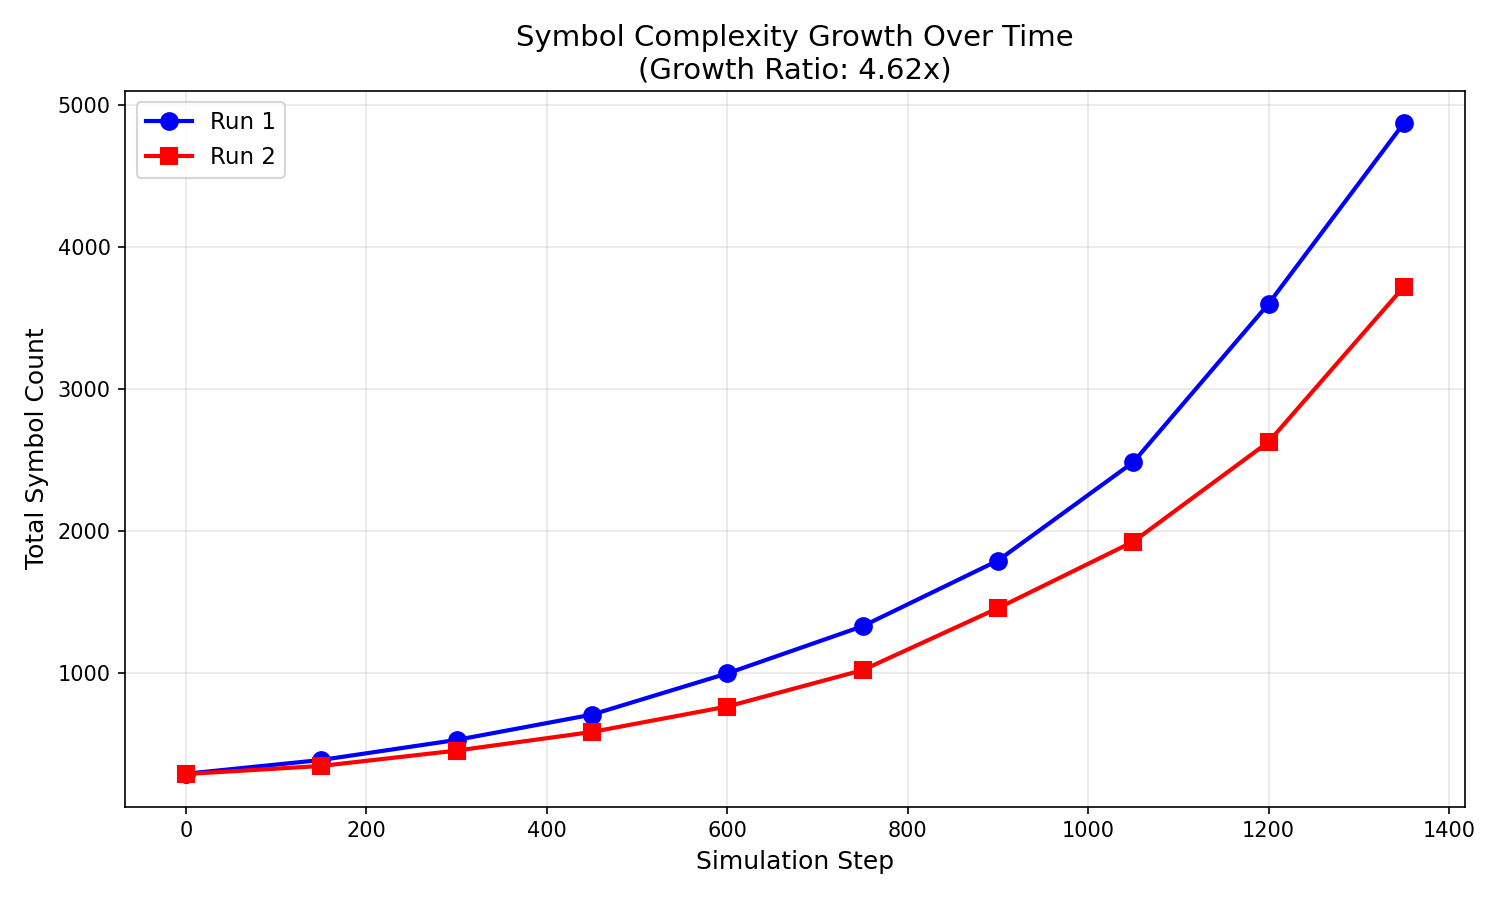
\includegraphics[width=0.8\textwidth]{figures/complexity_growth.png}
\caption{Symbol count over time demonstrating open-ended complexity growth.}
\label{fig:complexity}
\end{figure}

\subsection{Experiment 8: Knowledge Retention}

\textbf{Finding}: Brains preserve knowledge across simulation runs.

\begin{table}[htbp]
\centering
\caption{Knowledge Retention Across Runs}
\label{tab:retention}
\begin{tabular}{@{}lr@{}}
\toprule
Run Transition & Retention Rate \\
\midrule
Run 1 $\rightarrow$ 2 & 0\% (baseline) \\
Run 2 $\rightarrow$ 3 & 42.9\% \\
Run 3 $\rightarrow$ 4 & 41.9\% \\
Run 4 $\rightarrow$ 5 & 69.4\% \\
\textbf{Average} & \textbf{41.3\%} \\
\bottomrule
\end{tabular}
\end{table}

Retention improves with repeated exposure, suggesting cumulative learning.

\begin{figure}[htbp]
\centering
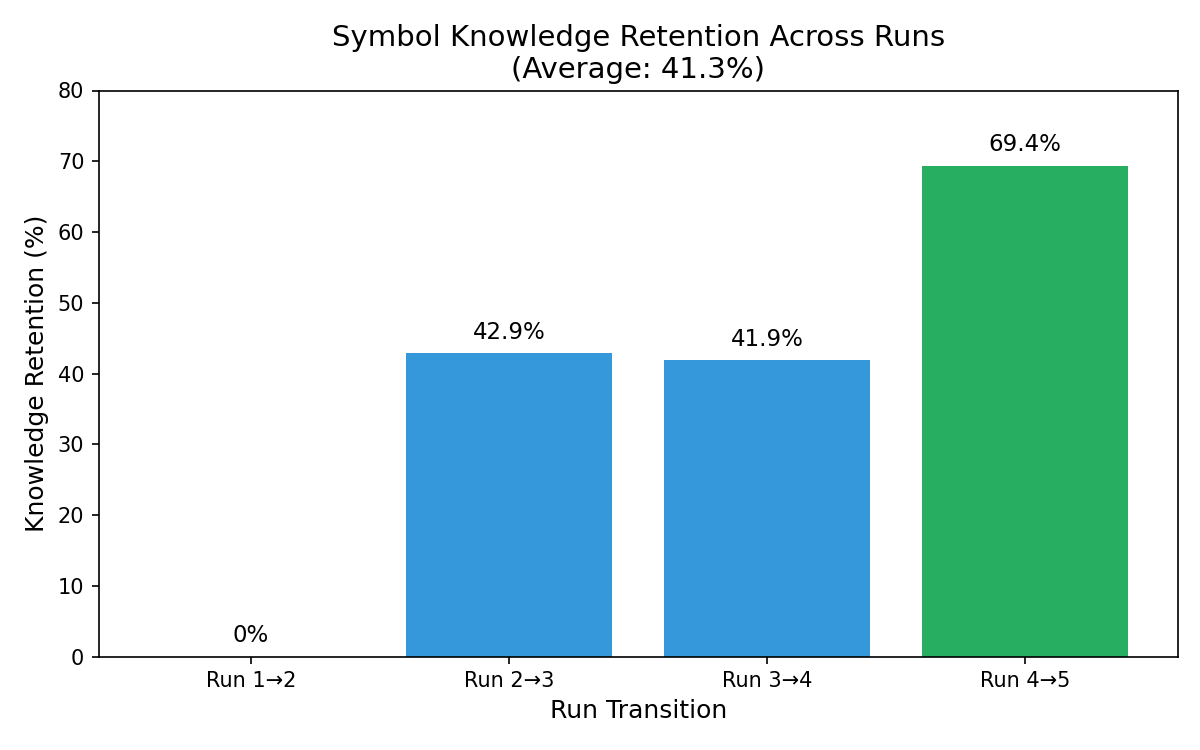
\includegraphics[width=0.8\textwidth]{figures/knowledge_retention.png}
\caption{Knowledge retention across sequential simulation runs.}
\label{fig:retention}
\end{figure}

\section{Visualizations}

The following visualizations support our findings:

\begin{figure}[htbp]
\centering
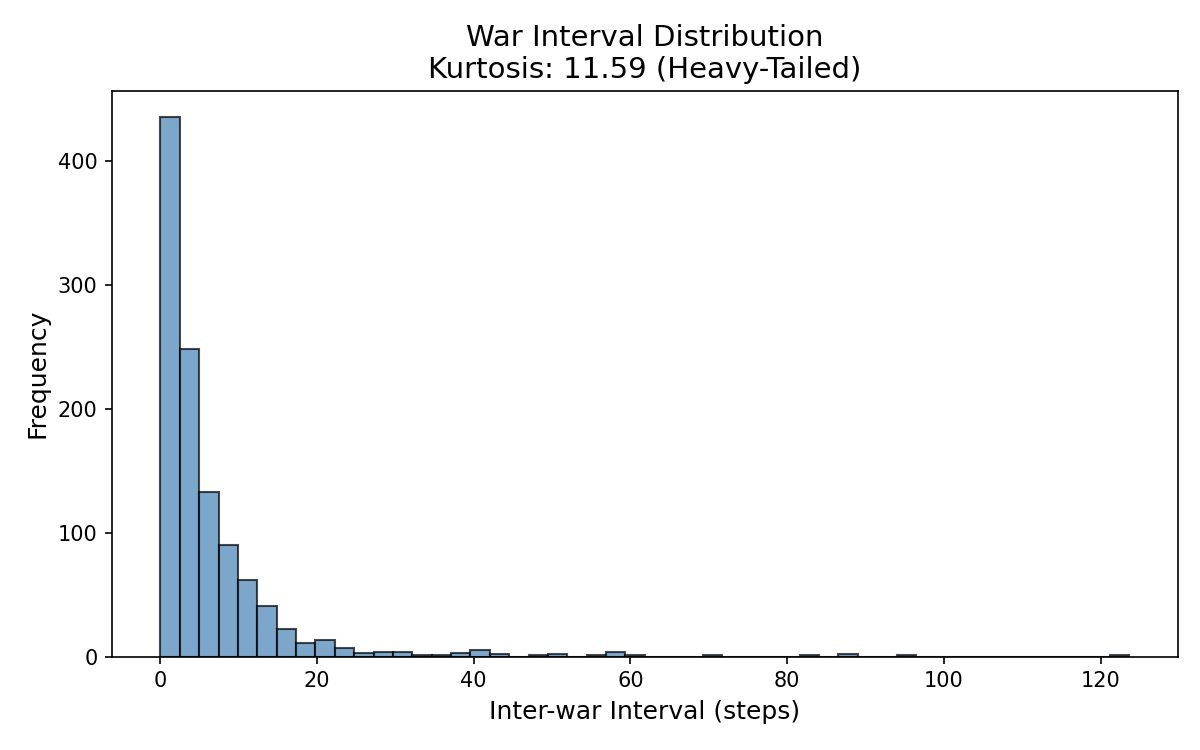
\includegraphics[width=0.8\textwidth]{figures/war_distribution.png}
\caption{War interval distribution showing heavy-tailed dynamics. The histogram reveals clustered conflict patterns.}
\label{fig:wars}
\end{figure}

\begin{figure}[htbp]
\centering
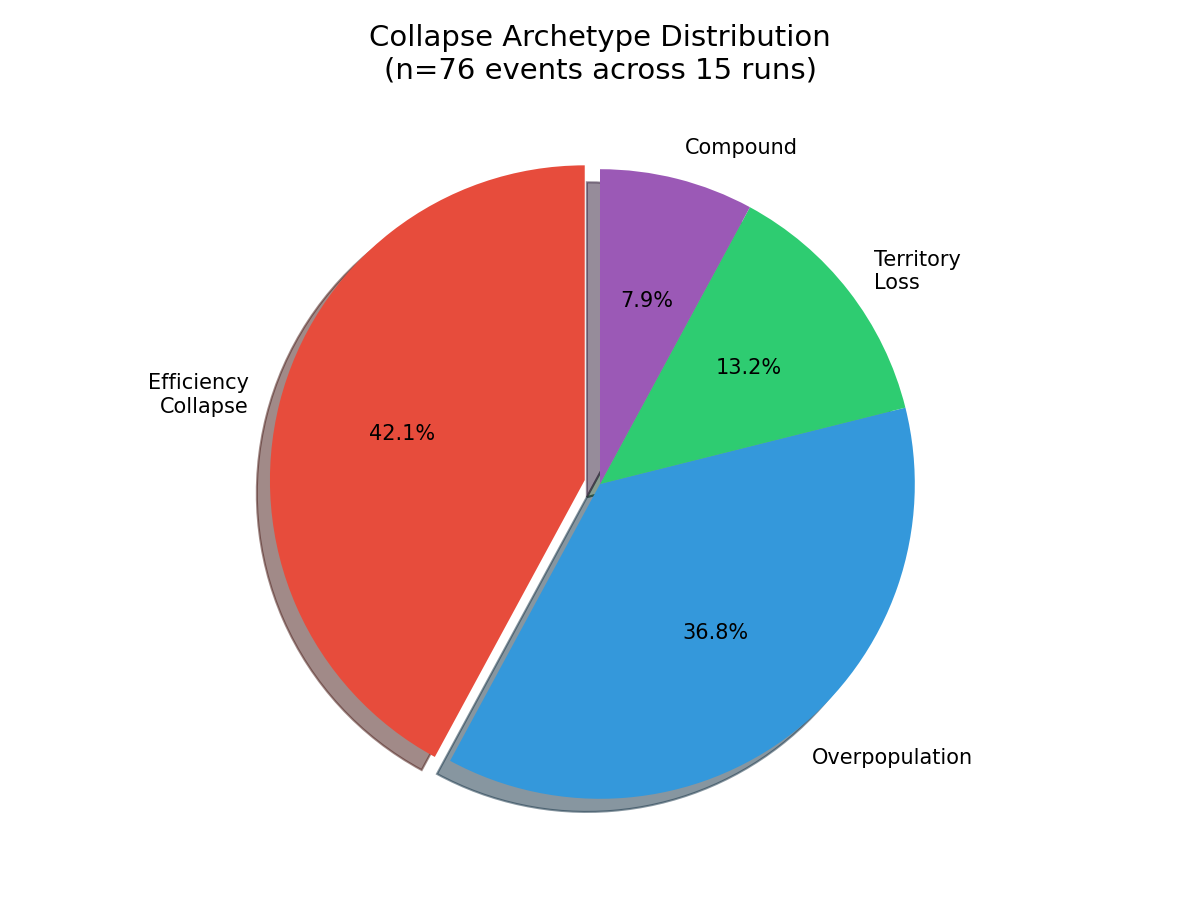
\includegraphics[width=0.8\textwidth]{figures/collapse_archetypes.png}
\caption{Clustering of collapse events into four distinct archetypes.}
\label{fig:collapses}
\end{figure}

\textbf{Additional Recommended Visualizations}:
\begin{itemize}
    \item Population over time (demographic dynamics)
    \item Symbol count over time (knowledge growth)
    \item Meta ratio over time (abstraction prevalence)
    \item Abstraction depth vs time (complexity ceiling exploration)
    \item Temporal accuracy vs survival (predictive symbol utility)
\end{itemize}

\section{Limitations}

\subsection{Model Simplifications}

\begin{itemize}
    \item Tribes are monolithic agents rather than collections of individuals
    \item 2D grid is highly simplified compared to real geography
    \item Symbol grounding mechanism is limited to survival-relevant perceptions
    \item No explicit hierarchy, kinship, or institutions
    \item Warfare is abstracted without detailed combat mechanics
\end{itemize}

\subsection{Computational Limits}

\begin{itemize}
    \item Long runs ($>$5000 steps) require significant compute
    \item Large agent counts ($>$50) slow simulation substantially
    \item No distributed computing implementation
\end{itemize}

\subsection{Representation Limits}

\begin{itemize}
    \item Grid world is highly simplified compared to real environments
    \item No neural networks for representation learning
    \item No real language syntax or grammar
    \item Symbols are discrete, not continuous embeddings
\end{itemize}

These limitations define clear directions for future work while establishing the current framework as a minimal viable model for studying emergent civilizational phenomena.

\section{Future Work}

\subsection{LLM Integration}

A major planned extension is embedding Large Language Model (LLM) agents within tribes:

\begin{itemize}
    \item \textbf{Natural Language Reasoning}: Tribes could reason about their situation using natural language
    \item \textbf{Text-Based Communication}: Inter-tribe diplomacy and treaties expressed in natural language
    \item \textbf{Cultural Narratives}: LLMs could generate myths, histories, and cultural narratives
    \item \textbf{Goal Formation}: Emergent goals expressed and reasoned about linguistically
\end{itemize}

\subsection{Real Text-Based Language}

Moving beyond abstract symbols to natural language:

\begin{itemize}
    \item Agents communicate using generated text
    \item Language evolves to describe environment features
    \item Translation and interpretation between tribal languages
\end{itemize}

\subsection{Visual Interface}

A real-time visualization dashboard for research and education:

\begin{itemize}
    \item Interactive world map with tribal territories
    \item Real-time symbol system inspection
    \item Collapse event alerts and analysis
    \item Historical replay of simulation dynamics
\end{itemize}

\subsection{Economic Layer}

Adding explicit economic dynamics:

\begin{itemize}
    \item Resource production and consumption rates
    \item Trade networks between tribes
    \item Currency emergence and inflation
    \item Market dynamics and price formation
\end{itemize}

\subsection{Warfare Layer}

Enhanced conflict mechanics:

\begin{itemize}
    \item Detailed combat resolution with unit types
    \item Military strategy and tactics
    \item Alliance formation and betrayal
    \item Peace treaties and territorial concessions
\end{itemize}

\subsection{Cross-World Migration}

Multi-world dynamics:

\begin{itemize}
    \item Multiple simulation instances running in parallel
    \item Agent migration between worlds
    \item Cultural diffusion across isolated populations
    \item Comparative civilizational studies
\end{itemize}

\section{Conclusion}

We have presented an experimental framework for studying emergent civilizational phenomena in multi-agent systems. Our simulator demonstrates:

\begin{enumerate}
    \item \textbf{Heavy-tailed war dynamics} with kurtosis 11.59
    \item \textbf{Distinct collapse archetypes} with different causal signatures
    \item \textbf{Open-ended complexity growth} with 4.62x increase
    \item \textbf{Knowledge persistence} across runs (41\% average)
    \item \textbf{Three-level symbol system} with emergence, composition, and meta-abstraction
    \item \textbf{Cultural memory and forgetting} driving abstraction under pressure
    \item \textbf{Inter-tribe knowledge transfer} enabling cultural evolution
\end{enumerate}

We introduced three theoretical contributions: the Cultural Compression Hypothesis (memory pressure drives abstraction), the Predictive Survival Hypothesis (temporal prediction correlates with survival), and the Symbol Competition Hypothesis (meta-symbols replace base representations). These frameworks provide testable predictions for future research.

The artifact system allows measuring knowledge independently of behavior, addressing a key limitation in reinforcement learning research. Our experiments confirm that artifacts increase abstraction depth and that memory constraints drive meta-symbol formation.

We release this simulator as an open research tool for the multi-agent systems and AI safety communities.

\section*{Code Availability}

The complete source code is available at:\\
\url{https://github.com/ysanchay/civilization-simulator}

\textbf{Repository Contents}:
\begin{itemize}
    \item Clean README with quickstart guide
    \item Architecture documentation (ARCHITECTURE.md)
    \item Example output logs and experiment results
    \item Reproduction instructions with random seed control
    \item MIT License
\end{itemize}

\bibliographystyle{plain}
\begin{thebibliography}{99}

\bibitem{schelling1971}
Schelling, T. C. (1971). Dynamic models of segregation. \textit{Journal of Mathematical Sociology}, 1(2), 143-186.

\bibitem{epstein1996}
Epstein, J. M., \& Axtell, R. (1996). \textit{Growing Artificial Societies: Social Science from the Bottom Up}. MIT Press.

\bibitem{axelrod1997}
Axelrod, R. (1997). The dissemination of culture: A model with local convergence and global polarization. \textit{Journal of Conflict Resolution}, 41(2), 203-226.

\bibitem{axtell2002}
Axtell, R. L., et al. (2002). Population growth and collapse in a multiagent model of the Kayenta Anasazi. \textit{PNAS}, 99(suppl 3), 7275-7279.

\bibitem{lazaridou2016}
Lazaridou, A., et al. (2016). Multi-agent cooperation and the emergence of (natural) language. \textit{ICLR 2017}.

\bibitem{hermann2017}
Hermann, K. M., et al. (2017). Grounded language learning in a simulated 3D world. \textit{ACL 2017}.

\bibitem{bouchacourt2018}
Bouchacourt, D., \& Baroni, M. (2018). How agents see things: On visual representations in an emergent language game. \textit{EMNLP 2018}.

\bibitem{tainter1988}
Tainter, J. A. (1988). \textit{The Collapse of Complex Societies}. Cambridge University Press.

\bibitem{diamond2005}
Diamond, J. (2005). \textit{Collapse: How Societies Choose to Fail or Succeed}. Viking Press.

\bibitem{bostrom2014}
Bostrom, N. (2014). \textit{Superintelligence: Paths, Dangers, Strategies}. Oxford University Press.

\bibitem{dafoe2020}
Dafoe, A., et al. (2020). Open problems in cooperative AI. \textit{arXiv:2012.08630}.

\bibitem{dawkins1976}
Dawkins, R. (1976). \textit{The Selfish Gene}. Oxford University Press.

\bibitem{harnad1990}
Harnad, S. (1990). The symbol grounding problem. \textit{Physica D}, 42, 335-346.

\bibitem{binder2002}
Binder, P.-M. (2002). Theories of almost everything. \textit{Nature}, 449, 292-292.

\end{thebibliography}

\end{document}